\chapter{Reduced Requirement set} \label{ch:Reduced Requirement Set}

\section{Turtlebot} %introduction
A Turtlebot is a prototype robot made for developers. In this project the Turtlebot will be used to test the different implementations which the project needs, due to the immense task of building a real rover in time for this project.\\
The Turtlebot consist of different parts, which will be described in this section.

\subsection{Base} %chassis
\begin{figure}[h]
    \centering
    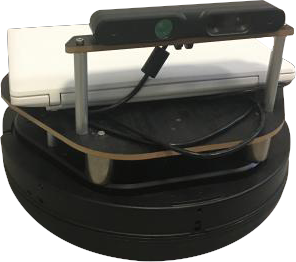
\includegraphics[width=.5\textwidth]{figures/turtlebot001.png}
    \caption{The turtlebot with new setup} 
    \label{fig:turtlebot} 
\end{figure}
The base is a Kobuki that is made for prototyping and educational use. The base has two motors, which can move the robot at a velocity of 0.65 m/s. The motors have an encoder on each wheel, which makes 11.5 ticks per millimetre of movement and 2578.33 ticks per full rotation. The motors are protected from high current above 3 amp. The maximum rotational velocity is 180 deg/s. The base has a gyro which works on the Z axis (110 deg/s calibrated from factory).\\
The base has three cliff sensors these sensors are located in the center and to left and right. The base has a wheel drop sensor that detect if a wheel has dropped into a hole. The Base wheels can drive over obstacles with a height of 12mm and the base can clear obstacle with a height of 15 mm. The base has two different batteries both on 14.8 VDC one has a capacity of 2200 mAh and the second one has a capacity of 4400 mAh.\\
The load capacity of the turtlebot is 5 kg on hard surface and on soft surfaces the load capacity is 4kg\cite{Base}.




\subsection{Computer} 
The computer is an ASUS notebook, it has an Intel core i3-4010U CPU that has 2 cores and operate at 1.7MHz\cite{CPU}. The notebook has 4GB RAM and an integrated HD graphics card on the motherboard\cite{ASUS}.
The operating system is Ubuntu 16.04 LTS a layer for the Linux distribution. For communication between the sensors and the Turtlebot, the computer uses USB 2.0.
\begin{figure}[h]
   \centering
    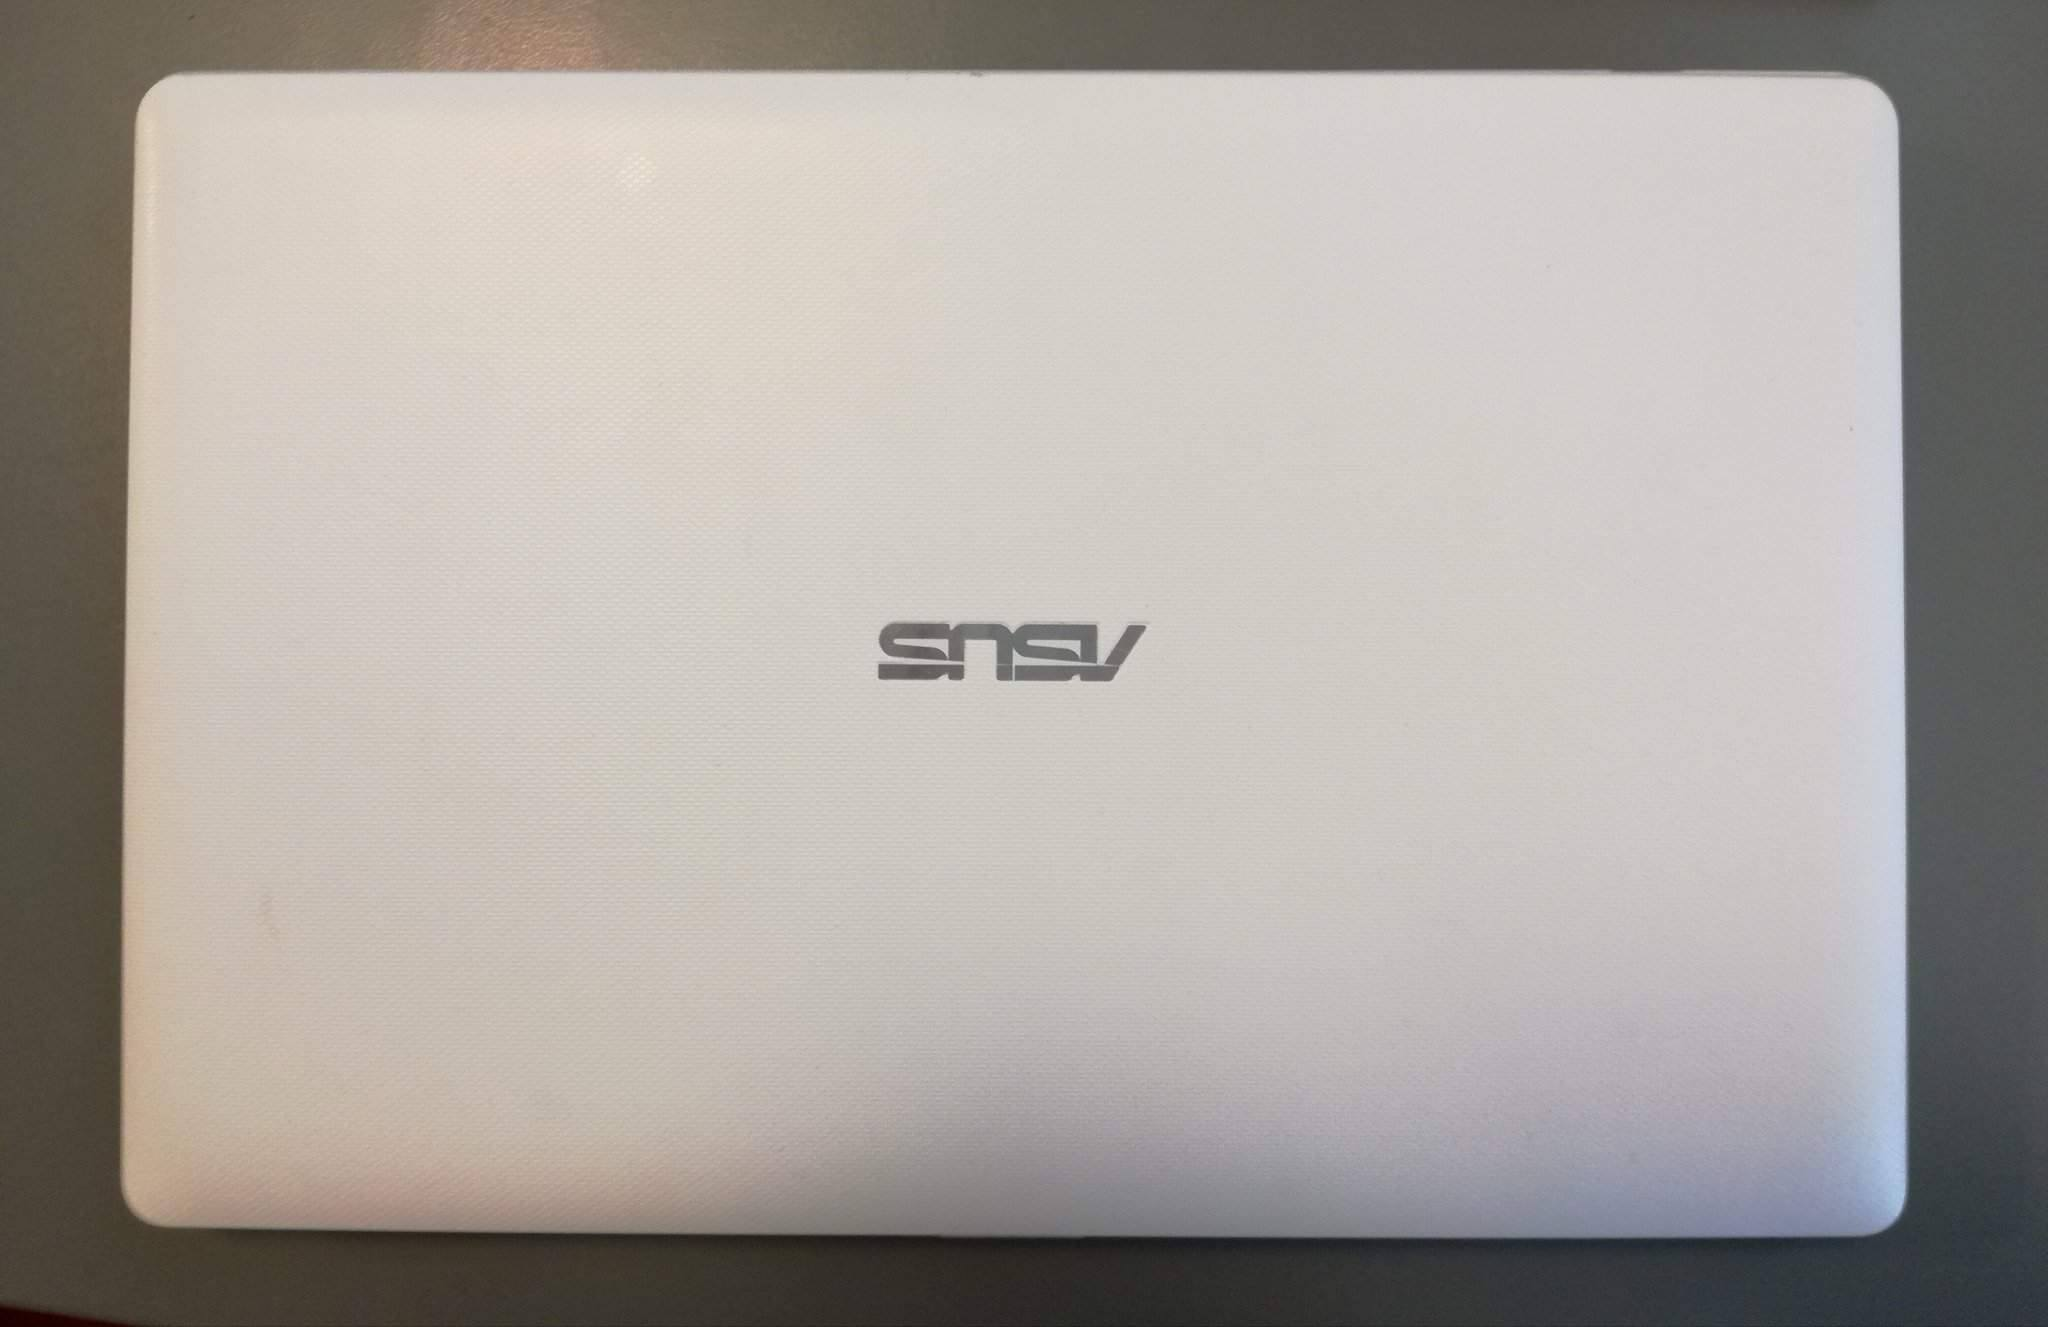
\includegraphics[width=.6\textwidth]{figures/ASUS.jpg}
    \caption{The computer that comes with the turtlebot}
    \label{fig:ASUS}
\end{figure}
